\documentclass[aspectratio=169,11pt]{beamer}

\usetheme{Madrid}
\usecolortheme{whale}
\usepackage[utf8]{inputenc}
\usepackage{booktabs}
\usepackage{amsmath}
\usepackage{graphicx}
\usepackage{tikz}
\usepackage{xcolor}
\usepackage{listings}
\usepackage{multicol}

% Custom colours
\definecolor{ucuBlue}{RGB}{0,51,102}
\definecolor{ucuGold}{RGB}{204,153,0}
\definecolor{lstmGreen}{RGB}{46,204,113}
\definecolor{arimaBlue}{RGB}{52,152,219}
\definecolor{prophetRed}{RGB}{231,76,60}
\definecolor{codebg}{RGB}{40,44,52}
\definecolor{codegreen}{RGB}{80,200,120}

\setbeamercolor{palette primary}{bg=ucuBlue,fg=white}
\setbeamercolor{palette secondary}{bg=ucuBlue!80,fg=white}
\setbeamercolor{palette tertiary}{bg=ucuBlue!60,fg=white}
\setbeamercolor{structure}{fg=ucuBlue}
\setbeamercolor{block title}{bg=ucuBlue,fg=white}
\setbeamercolor{block body}{bg=ucuBlue!5}

\setbeamertemplate{navigation symbols}{}
\setbeamertemplate{footline}[frame number]

% Code listing style
\lstset{
    language=Python,
    basicstyle=\tiny\ttfamily\color{white},
    keywordstyle=\color{codegreen}\bfseries,
    stringstyle=\color{orange},
    commentstyle=\color{gray},
    backgroundcolor=\color{codebg},
    frame=single,
    rulecolor=\color{gray!50},
    breaklines=true,
    showstringspaces=false,
    numbers=none,
    xleftmargin=4pt,
    xrightmargin=4pt,
    aboveskip=4pt,
    belowskip=4pt,
}

\title[Crop Price Forecasting]{\textbf{Market Price Forecasting for\\Ugandan Staple Crops}}
\subtitle{A Multi-Model Time-Series Approach Using WFP Market Data and Climate Covariates}
\author[Group 3]{
    Jamugisa Peter Paul \textnormal{(B35503 -- S25M25/008)} \\
    ILEGO Cynthia Cecilia \textnormal{(B35502 -- S25M25/007)} \\
    AYEBARE Moses \textnormal{(B35498 -- S25M25/003)} \\
    Apilli Barbra Ebal \textnormal{(B35496 -- S25M25/001)}
}
\institute[UCU]{
    Department of Computer Science $\bullet$ Uganda Christian University \\
    \textit{MSc Computer Science -- AI \& Machine Learning}
}
\date{April 2025}

\begin{document}

% ============================================================
% TITLE SLIDE
% ============================================================
\begin{frame}
\titlepage
\end{frame}

% ============================================================
% OUTLINE
% ============================================================
\begin{frame}{Presentation Outline}
\small
\begin{columns}
\begin{column}{0.48\textwidth}
\textbf{Presenter 1 -- Jamugisa Peter Paul}
\begin{itemize}
    \item[\S1] Introduction \& Problem Statement
    \item[\S2] The Data Pipeline
\end{itemize}
\vspace{0.5em}
\textbf{Presenter 2 -- ILEGO Cynthia Cecilia}
\begin{itemize}
    \item[\S3] Feature Engineering
    \item[\S4] Model 1: ARIMA Baseline
\end{itemize}
\end{column}
\begin{column}{0.48\textwidth}
\textbf{Presenter 3 -- AYEBARE Moses}
\begin{itemize}
    \item[\S5] Model 2: Facebook Prophet
    \item[\S6] Model 3: LSTM Neural Network
\end{itemize}
\vspace{0.5em}
\textbf{Presenter 4 -- Apilli Barbra Ebal}
\begin{itemize}
    \item[\S7] Results \& Model Comparison
    \item[\S8] Live Dashboard Demo
    \item[\S9] Challenges \& Conclusions
\end{itemize}
\end{column}
\end{columns}
\end{frame}

% ============================================================
% SECTION 1: INTRODUCTION (Presenter 1 - Jamugisa Peter Paul)
% ============================================================
\section{Introduction \& Problem Statement}

\begin{frame}{The Problem: Food Insecurity through Price Volatility}
\textit{\small Presenter: Jamugisa Peter Paul \hfill [0:00 -- 2:30]}
\vspace{0.3em}
\begin{columns}
\begin{column}{0.52\textwidth}
\begin{itemize}
    \item Agriculture = \textbf{24\% of Uganda's GDP}
    \item Employs \textbf{70\%+} of the workforce
    \item Staple crops: \textbf{Maize, Beans, Cassava}
    \item Prices fluctuate \textbf{30--50\%} between seasons
    \item Existing WFP/FEWS NET systems are \textbf{retrospective} -- they tell us what prices \textit{are}, not what they \textit{will be}
\end{itemize}
\vspace{0.3em}
\begin{block}{Our Solution}
Build a machine learning system that forecasts crop prices \textbf{4--8 weeks ahead} at district level
\end{block}
\end{column}
\begin{column}{0.45\textwidth}
\begin{block}{Impact for Stakeholders}
\begin{itemize}
    \item[\checkmark] \textbf{Farmers} optimise selling timing
    \item[\checkmark] \textbf{NGOs} pre-position food aid
    \item[\checkmark] \textbf{Policymakers} plan interventions
\end{itemize}
\end{block}
\vspace{0.3em}
\begin{alertblock}{Research Question}
\small\textit{Which model -- ARIMA, Prophet, or LSTM -- forecasts best when rainfall is a predictor?}
\end{alertblock}
\end{column}
\end{columns}
\end{frame}

\begin{frame}{Research Objectives}
\textit{\small Presenter: Jamugisa Peter Paul}
\begin{enumerate}
    \item \textbf{Collect \& Merge} WFP prices + CHIRPS rainfall + World Bank commodity indices
    \item \textbf{Engineer Features:} lags, rolling stats, seasonal encoding, climate covariates
    \item \textbf{Implement 3 Models:} ARIMA, Facebook Prophet, LSTM
    \item \textbf{Evaluate \& Compare} using MAE, RMSE, MAPE (80/20 chronological split)
    \item \textbf{Deploy} best model in an interactive Streamlit dashboard
\end{enumerate}
\vspace{0.5em}
\begin{block}{Scope}
\centering
\begin{tabular}{ccc}
\textbf{3 Crops} & \textbf{3 Districts} & \textbf{14 Years} \\
Maize, Beans, Cassava & Kampala, Gulu, Mbale & 2010--2024 \\
\end{tabular}
\end{block}
\end{frame}

% ============================================================
% SECTION 2: DATA PIPELINE (Presenter 1 continued)
% ============================================================
\section{The Data Pipeline}

\begin{frame}{Three Heterogeneous Data Sources}
\textit{\small Presenter: Jamugisa Peter Paul \hfill [2:30 -- 5:00]}
\begin{table}
\centering
\small
\begin{tabular}{p{2.8cm}p{3.5cm}p{3.5cm}p{2.8cm}}
\toprule
\textbf{Dataset} & \textbf{Source} & \textbf{Content} & \textbf{Role} \\
\midrule
WFP Food Prices & Humanitarian Data Exchange & Market prices (UGX) across districts & \textbf{Target variable} \\
\midrule
CHIRPS Rainfall & UC Santa Barbara satellite & Monthly rainfall (mm) by region & \textbf{Climate covariate} \\
\midrule
World Bank Commodities & World Bank & Global crude oil \& maize indices & \textbf{Global proxy} \\
\bottomrule
\end{tabular}
\end{table}

\begin{block}{Why These Three?}
\begin{itemize}
    \item \textbf{Rainfall:} Uganda's agriculture is rain-fed -- drought today = high prices in 4 months
    \item \textbf{Crude Oil:} Drives transport costs on Uganda's unpaved roads
    \item \textbf{Global Maize:} International supply-demand spills into local markets via trade
\end{itemize}
\end{block}
\end{frame}

\begin{frame}{Price Trends Across All Crop-District Pairs}
\textit{\small Presenter: Jamugisa Peter Paul \hfill [5:00 -- 5:45]}
\begin{center}
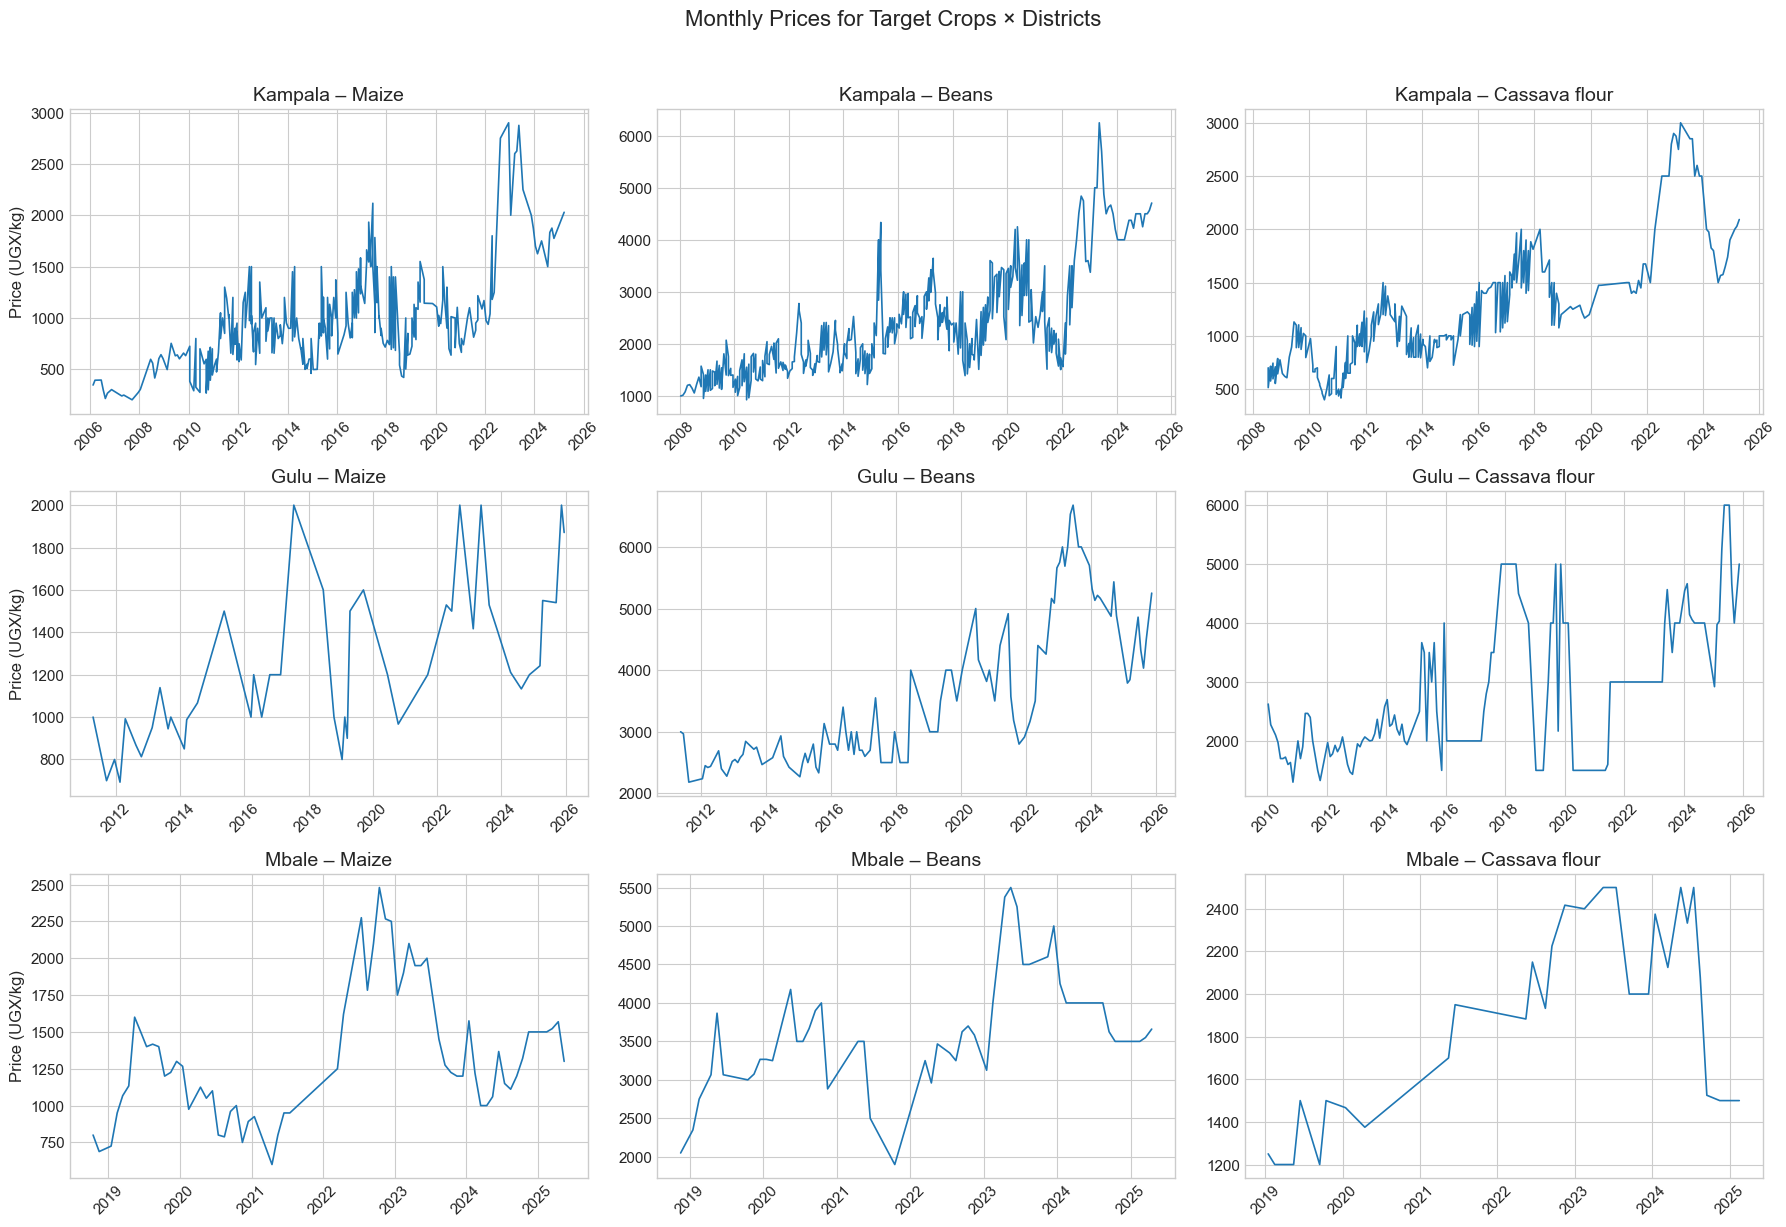
\includegraphics[width=0.82\textwidth]{slides_img/plot_00.png}
\end{center}
\vspace{-0.3cm}
\footnotesize\textit{3$\times$3 grid: Maize, Beans, Cassava flour across Kampala, Gulu, Mbale (2010--2024)}
\end{frame}

\begin{frame}{Rainfall Patterns \& World Bank Commodity Trends}
\textit{\small Presenter: Jamugisa Peter Paul \hfill [5:45 -- 7:00]}
\begin{columns}
\begin{column}{0.48\textwidth}
\begin{center}
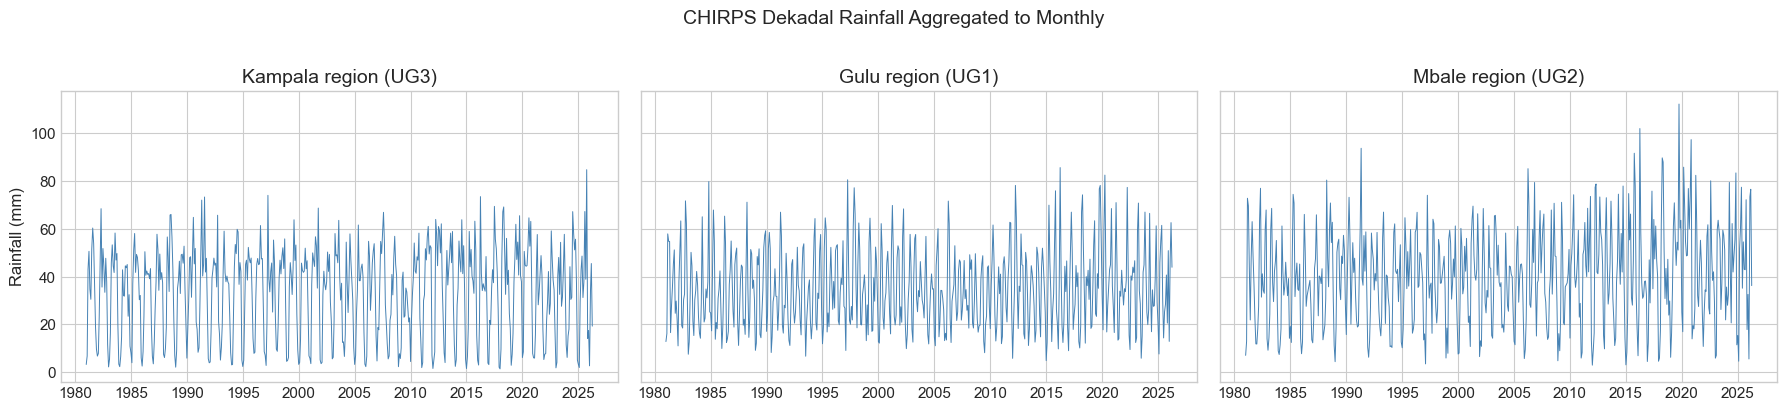
\includegraphics[width=\textwidth]{slides_img/plot_01.png}
\end{center}
\footnotesize\textit{CHIRPS rainfall by region -- clear bimodal wet season pattern}
\end{column}
\begin{column}{0.48\textwidth}
\begin{center}
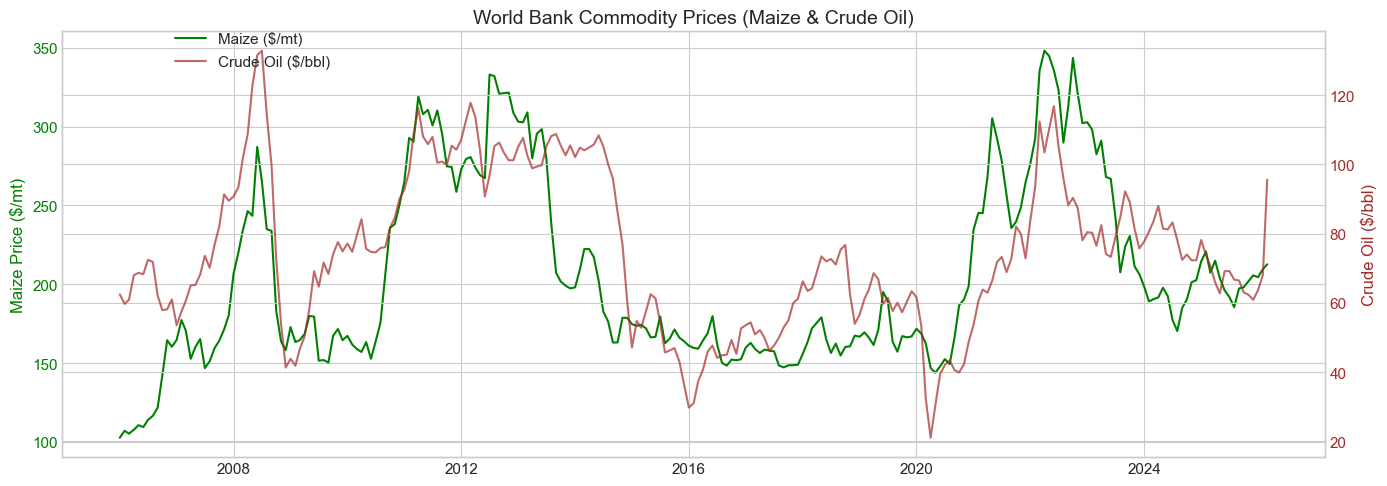
\includegraphics[width=\textwidth]{slides_img/plot_02.png}
\end{center}
\footnotesize\textit{Global crude oil \& maize prices -- transport cost proxies}
\end{column}
\end{columns}
\end{frame}

% ============================================================
% SECTION 3: FEATURE ENGINEERING (Presenter 2 - Cynthia)
% ============================================================
\section{Feature Engineering}

\begin{frame}{Transforming Raw Data into AI-Ready Features}
\textit{\small Presenter: ILEGO Cynthia Cecilia \hfill [7:00 -- 10:00]}
\begin{columns}
\begin{column}{0.48\textwidth}
\begin{block}{1. Price Lag Features}
$$\text{price\_lag}_k(t) = \text{price}(t - k)$$
$k \in \{1, 2, 4, 8\}$ -- captures momentum
\end{block}

\begin{block}{2. Rolling Statistics}
$$\text{roll\_mean}_w = \frac{1}{w}\sum_{i=0}^{w-1} \text{price}(t-i)$$
Windows: 4 \& 8 months (mean + std dev)
\end{block}
\end{column}
\begin{column}{0.48\textwidth}
\begin{block}{3. Sinusoidal Seasonal Encoding}
$$\text{month\_sin} = \sin\!\left(\frac{2\pi m}{12}\right)$$
$$\text{month\_cos} = \cos\!\left(\frac{2\pi m}{12}\right)$$
\footnotesize Preserves cyclical continuity (Dec $\leftrightarrow$ Jan)
\end{block}

\begin{block}{4. Climate \& Global Lags}
$$\text{rain\_lag}_k(t) = \text{rainfall}(t - k)$$
$k \in \{1, 4, 8\}$ + WB oil \& maize indices
\end{block}
\end{column}
\end{columns}
\end{frame}

\begin{frame}{Feature Analysis: Correlation \& Seasonality}
\textit{\small Presenter: ILEGO Cynthia Cecilia}
\begin{columns}
\begin{column}{0.48\textwidth}
\begin{center}
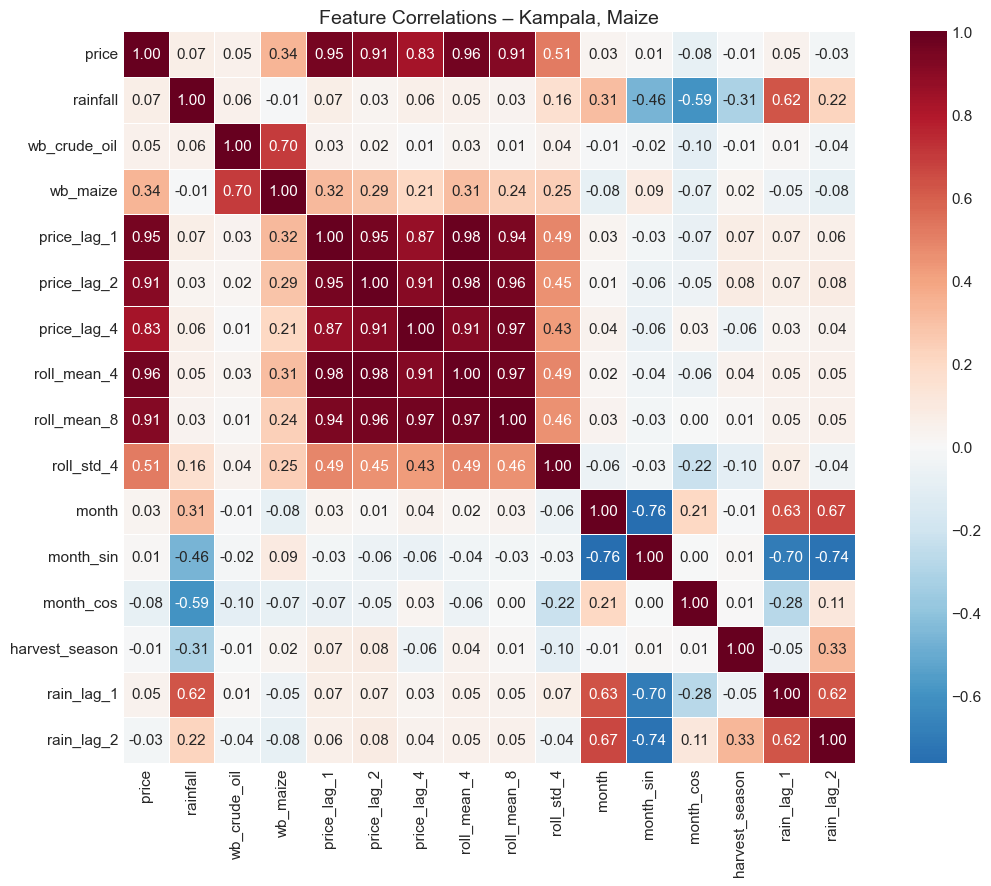
\includegraphics[width=\textwidth]{slides_img/plot_04.png}
\end{center}
\footnotesize\textit{Correlation heatmap -- strong lag autocorrelation confirms feature selection}
\end{column}
\begin{column}{0.48\textwidth}
\begin{center}
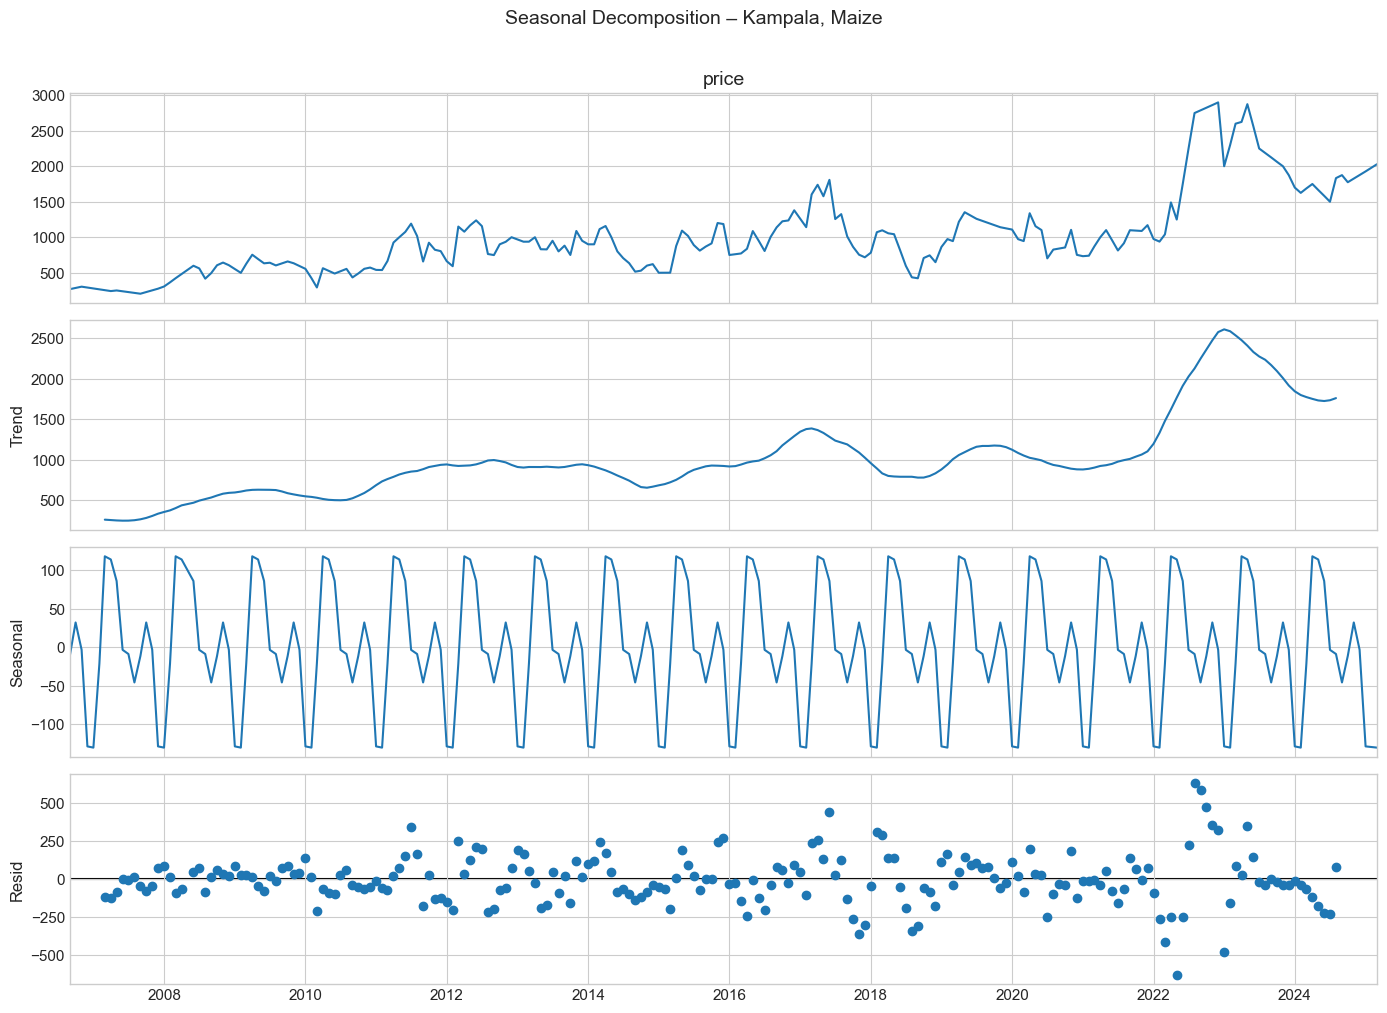
\includegraphics[width=\textwidth]{slides_img/plot_05.png}
\end{center}
\footnotesize\textit{Seasonal decomposition -- clear yearly pattern validates seasonal encoding}
\end{column}
\end{columns}
\end{frame}

% ============================================================
% SECTION 4: ARIMA (Presenter 2 continued)
% ============================================================
\section{Model 1: ARIMA Baseline}

\begin{frame}[fragile]{ARIMA: Classical Statistical Baseline}
\textit{\small Presenter: ILEGO Cynthia Cecilia \hfill [10:00 -- 12:30]}
\begin{columns}
\begin{column}{0.55\textwidth}
\textbf{ARIMA(p, d, q) equation:}
$$y'_t = c + \sum_{i=1}^{p}\phi_i y'_{t-i} + \sum_{j=1}^{q}\theta_j \varepsilon_{t-j} + \varepsilon_t$$

\begin{itemize}
    \item \textbf{AR($p$):} Linear combination of $p$ past values
    \item \textbf{I($d$):} Differencing for stationarity
    \item \textbf{MA($q$):} Past forecast errors for self-correction
\end{itemize}
\vspace{0.3em}
\textbf{Order Selection:} AIC grid search
$$\text{AIC} = 2k - 2\ln(\hat{L})$$
$p \in \{0..3\}$, $d \in \{0,1\}$, $q \in \{0..3\}$ = 32 candidates
\end{column}
\begin{column}{0.42\textwidth}
\begin{lstlisting}
# ARIMA AIC Grid Search
from statsmodels.tsa.statespace
    .sarimax import SARIMAX

best_aic = float('inf')
for p in range(4):
  for d in range(2):
    for q in range(4):
      model = SARIMAX(
        train['price'],
        order=(p, d, q))
      result = model.fit(
        disp=False)
      if result.aic < best_aic:
        best_aic = result.aic
        best_order = (p, d, q)
\end{lstlisting}
\end{column}
\end{columns}
\end{frame}

\begin{frame}{ARIMA Forecast Results}
\textit{\small Presenter: ILEGO Cynthia Cecilia \hfill [12:30 -- 14:00]}
\begin{center}
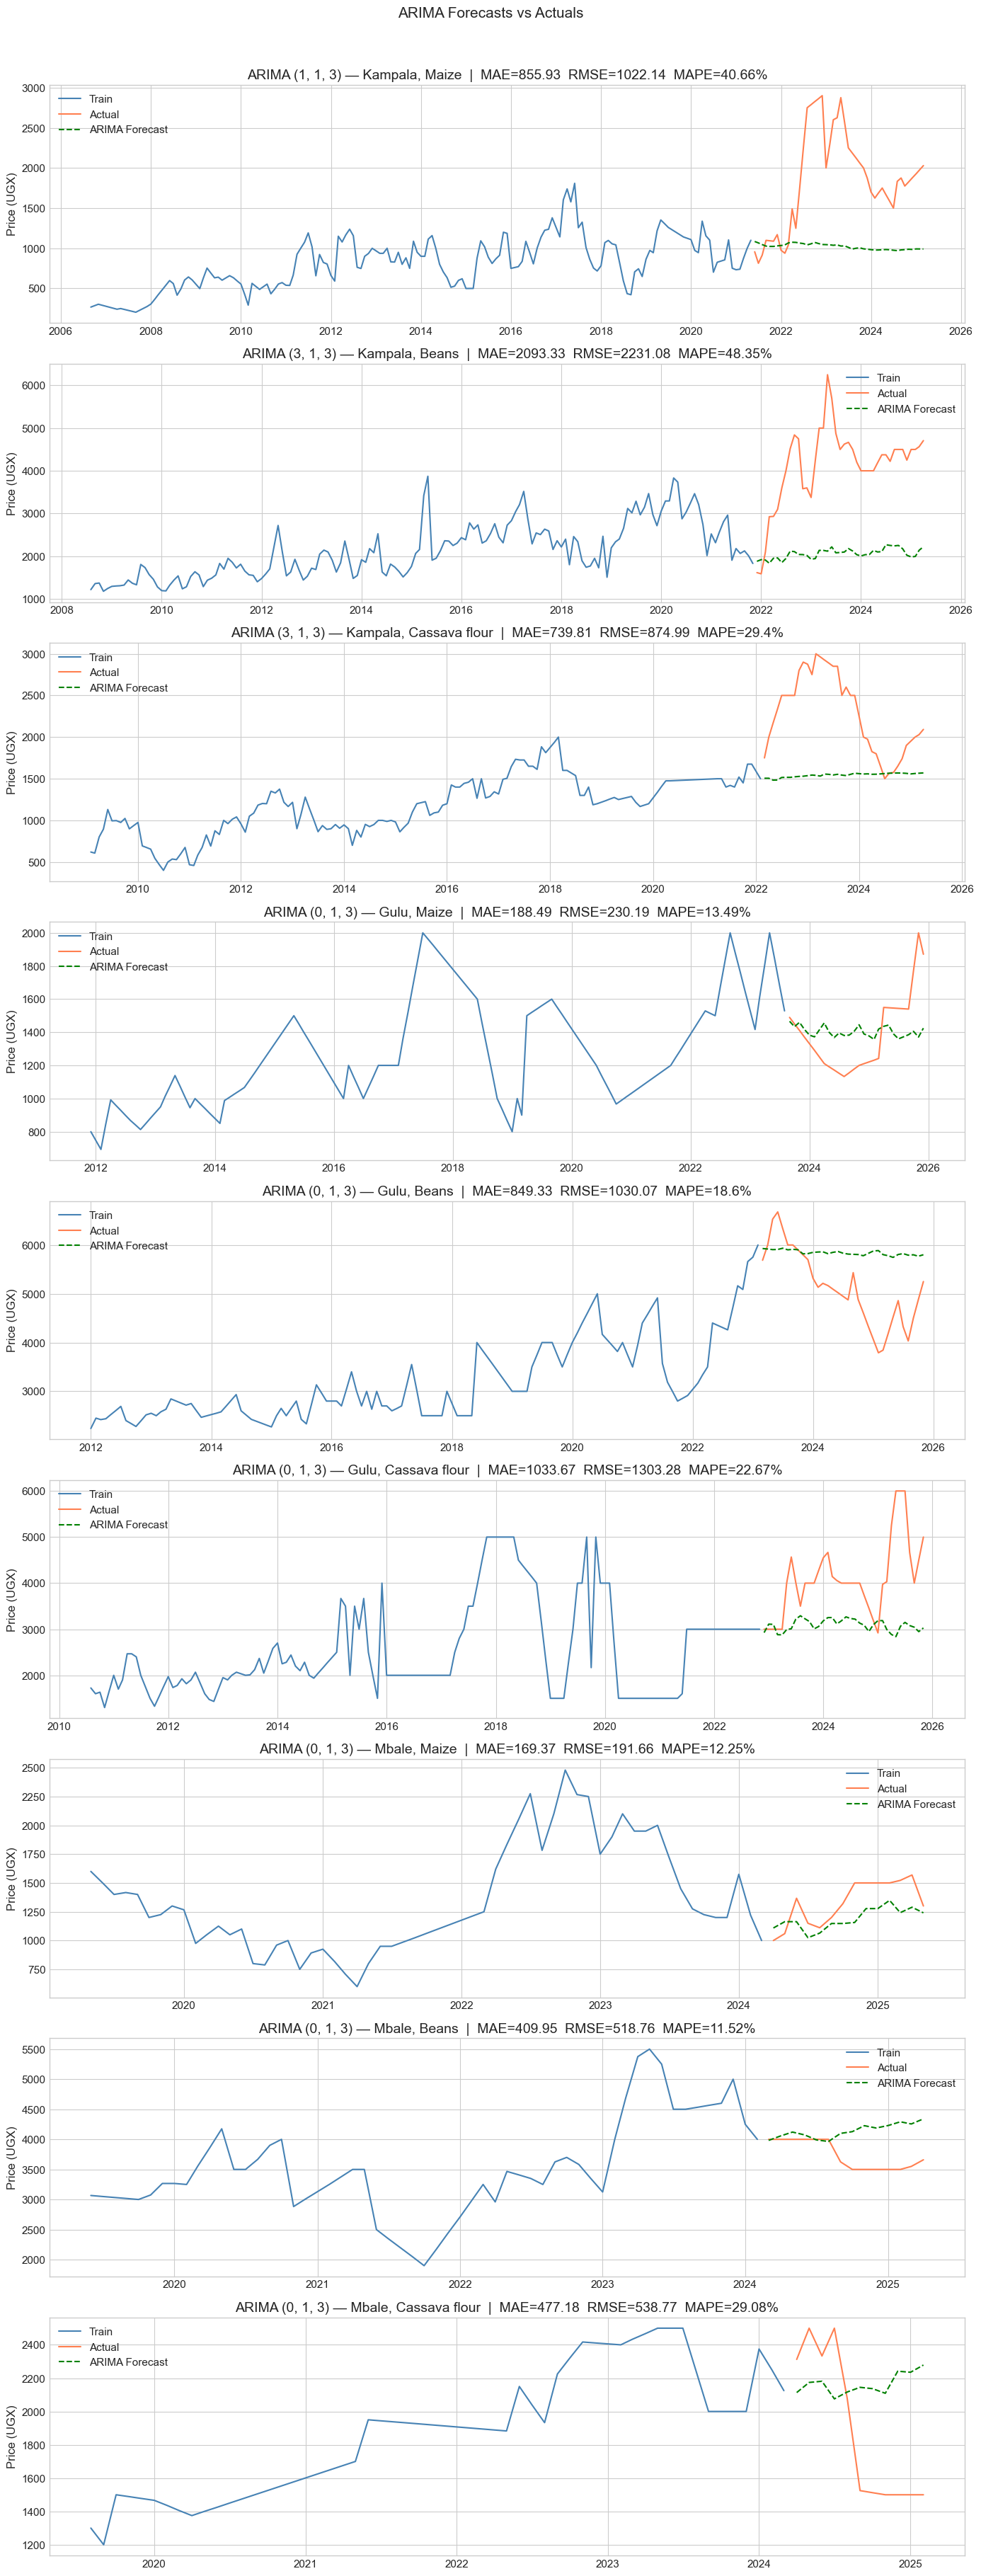
\includegraphics[width=0.78\textwidth]{slides_img/plot_09.png}
\end{center}
\vspace{-0.3cm}
\footnotesize\textit{ARIMA forecasts (dashed red) vs actuals (blue) across all 9 crop-district pairs. Average MAPE: \textbf{25.11\%}}
\end{frame}

% ============================================================
% SECTION 5: PROPHET (Presenter 3 - Moses)
% ============================================================
\section{Model 2: Facebook Prophet}

\begin{frame}[fragile]{Prophet: Additive Decomposition with Rainfall}
\textit{\small Presenter: AYEBARE Moses \hfill [14:00 -- 16:00]}
\begin{columns}
\begin{column}{0.55\textwidth}
\textbf{Prophet Decomposition:}
$$y(t) = g(t) + s(t) + \beta_{\text{rain}} \cdot \text{rainfall}(t) + \varepsilon_t$$

\begin{itemize}
    \item $g(t)$ = \textbf{Piecewise linear trend} with automatic changepoint detection
    \item $s(t)$ = \textbf{Fourier seasonal component}:
    $$s(t) = \sum_{n=1}^{N}\!\left(a_n\cos\frac{2\pi nt}{P} + b_n\sin\frac{2\pi nt}{P}\right)$$
    \item $\beta_{\text{rain}}$ = Learned rainfall coefficient
\end{itemize}
\end{column}
\begin{column}{0.42\textwidth}
\begin{lstlisting}
# Prophet with Rainfall
from prophet import Prophet

m = Prophet(
    yearly_seasonality=True,
    weekly_seasonality=False,
    daily_seasonality=False)

# Add rainfall as regressor
m.add_regressor('rainfall')
m.fit(train_df)

future = m.make_future_dataframe(
    periods=len(test))
forecast = m.predict(future)
\end{lstlisting}
\end{column}
\end{columns}
\end{frame}

\begin{frame}{Prophet: Results \& Component Decomposition}
\textit{\small Presenter: AYEBARE Moses \hfill [16:00 -- 17:30]}
\begin{columns}
\begin{column}{0.55\textwidth}
\begin{center}
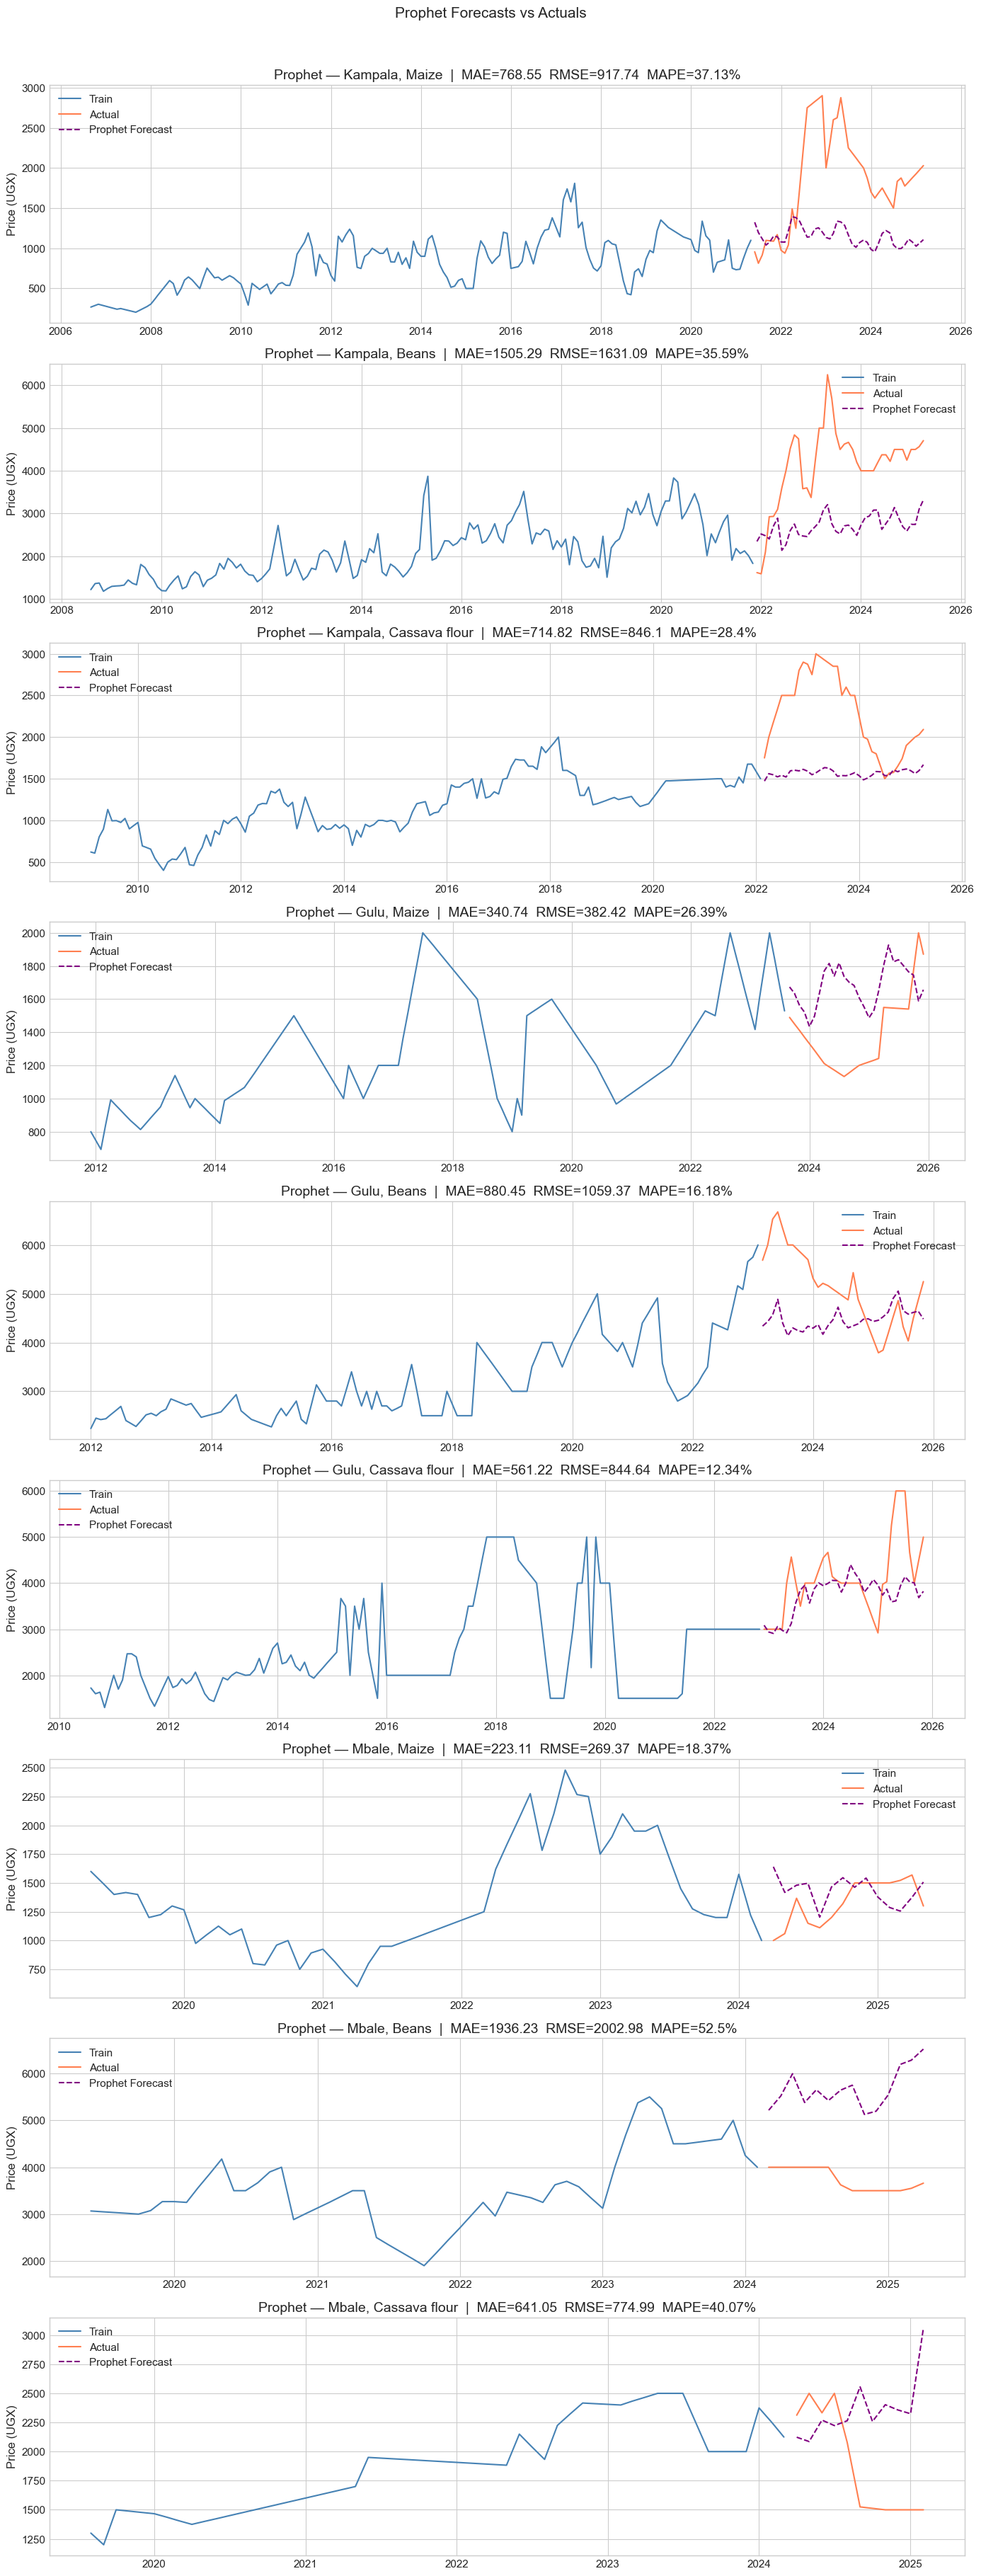
\includegraphics[width=\textwidth]{slides_img/plot_10.png}
\end{center}
\vspace{-0.2cm}
\footnotesize\textit{Prophet forecasts -- average MAPE: \textbf{29.66\%}}
\end{column}
\begin{column}{0.42\textwidth}
\begin{center}
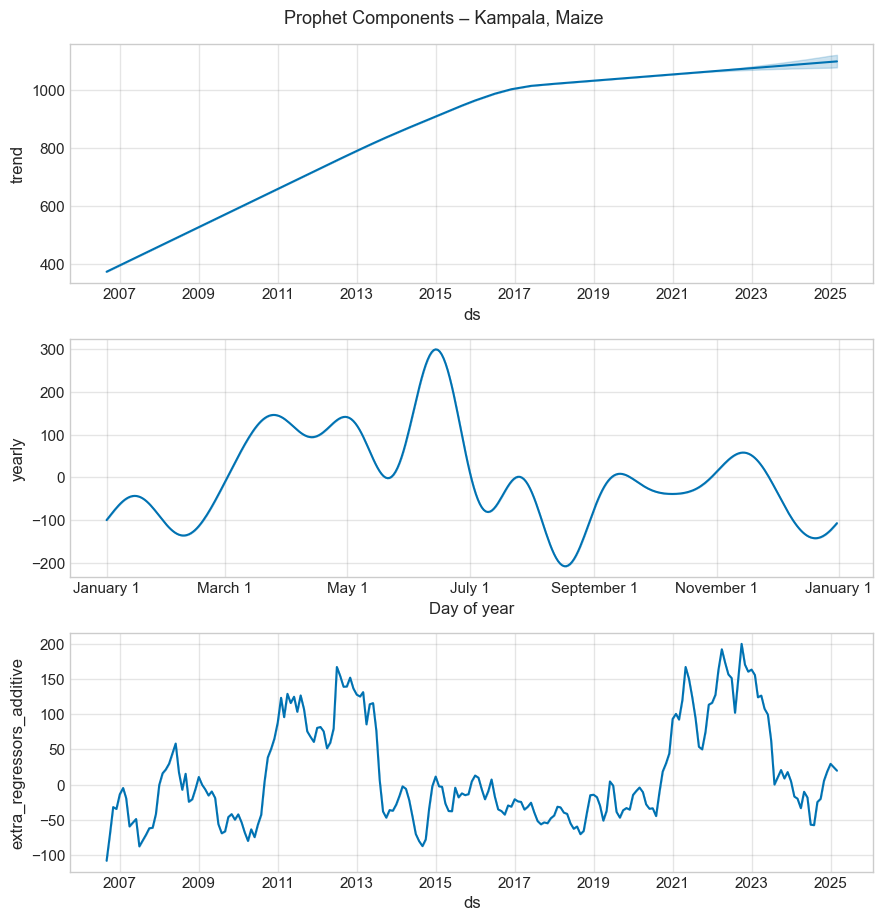
\includegraphics[width=\textwidth]{slides_img/plot_11.png}
\end{center}
\vspace{-0.2cm}
\footnotesize\textit{Prophet component decomposition: trend, seasonality, rainfall}

\vspace{0.3em}
\begin{alertblock}{\small Why Prophet Underperformed}
\footnotesize
\begin{itemize}
    \item Spurious changepoint detection
    \item Fixed Fourier seasonality vs shifting Ugandan harvests
    \item Designed for business data, not agriculture
\end{itemize}
\end{alertblock}
\end{column}
\end{columns}
\end{frame}

% ============================================================
% SECTION 6: LSTM (Presenter 3 continued)
% ============================================================
\section{Model 3: LSTM Neural Network}

\begin{frame}{LSTM: Deep Learning Architecture}
\textit{\small Presenter: AYEBARE Moses \hfill [17:30 -- 20:00]}
\begin{columns}
\begin{column}{0.55\textwidth}
\textbf{LSTM Gating Mechanism:}
\begin{align*}
f_t &= \sigma(W_f \cdot [h_{t-1}, x_t] + b_f) & \text{\footnotesize Forget}\\
i_t &= \sigma(W_i \cdot [h_{t-1}, x_t] + b_i) & \text{\footnotesize Input}\\
o_t &= \sigma(W_o \cdot [h_{t-1}, x_t] + b_o) & \text{\footnotesize Output}\\
C_t &= f_t \odot C_{t-1} + i_t \odot \tilde{C}_t & \text{\footnotesize Cell State}
\end{align*}
\vspace{-0.3em}
\begin{itemize}
    \item Cell state = \textbf{``memory highway''} -- carries information across time steps
    \item Solves \textbf{vanishing gradient problem} of standard RNNs
\end{itemize}
\end{column}
\begin{column}{0.42\textwidth}
\begin{block}{\small Our Architecture}
\footnotesize
\begin{tabular}{ll}
\textbf{Layer 1} & LSTM (64 units) \\
\textbf{Dropout} & 20\% \\
\textbf{Layer 2} & LSTM (32 units) \\
\textbf{Dropout} & 20\% \\
\textbf{Output} & Dense (1 unit) \\
\midrule
\textbf{Window} & 6 months \\
\textbf{Features} & 9 inputs \\
\textbf{Optimiser} & Adam \\
\textbf{Loss} & MSE \\
\textbf{Epochs} & 100 (early stop) \\
\end{tabular}
\end{block}
\end{column}
\end{columns}
\end{frame}

\begin{frame}[fragile]{LSTM: Implementation \& Training Code}
\textit{\small Presenter: AYEBARE Moses \hfill [20:00 -- 21:00]}
\begin{columns}
\begin{column}{0.48\textwidth}
\begin{lstlisting}
# LSTM Architecture (TensorFlow/Keras)
from tensorflow.keras.models import Sequential
from tensorflow.keras.layers import (
    LSTM, Dense, Dropout)

model = Sequential([
    LSTM(64, return_sequences=True,
         input_shape=(6, 9)),
    Dropout(0.2),
    LSTM(32, return_sequences=False),
    Dropout(0.2),
    Dense(1)  # Price prediction
])

model.compile(
    optimizer='adam', loss='mse')

model.fit(X_train, y_train,
    epochs=100, batch_size=16,
    callbacks=[EarlyStopping(
        patience=10)])
\end{lstlisting}
\end{column}
\begin{column}{0.48\textwidth}
\begin{lstlisting}
# 9-Feature Input Vector
LSTM_FEATURES = [
    'price',        # Current
    'rainfall',     # Climate
    'wb_crude_oil', # Global oil
    'wb_maize',     # Global maize
    'price_lag_1',  # 1 month ago
    'price_lag_2',  # 2 months ago
    'month_sin',    # Seasonal
    'month_cos',    # Seasonal
    'rain_lag_1'    # Rain 1mo ago
]

# MinMax Normalisation
scaler = MinMaxScaler()
train_sc = scaler.fit_transform(
    train[LSTM_FEATURES])

# Sliding Window: 6 months -> 1
X, y = create_sequences(
    train_sc, window=6)
\end{lstlisting}
\end{column}
\end{columns}
\end{frame}

\begin{frame}{LSTM: Training Curves \& Forecast Results}
\textit{\small Presenter: AYEBARE Moses \hfill [21:00 -- 22:00]}
\begin{columns}
\begin{column}{0.48\textwidth}
\begin{center}
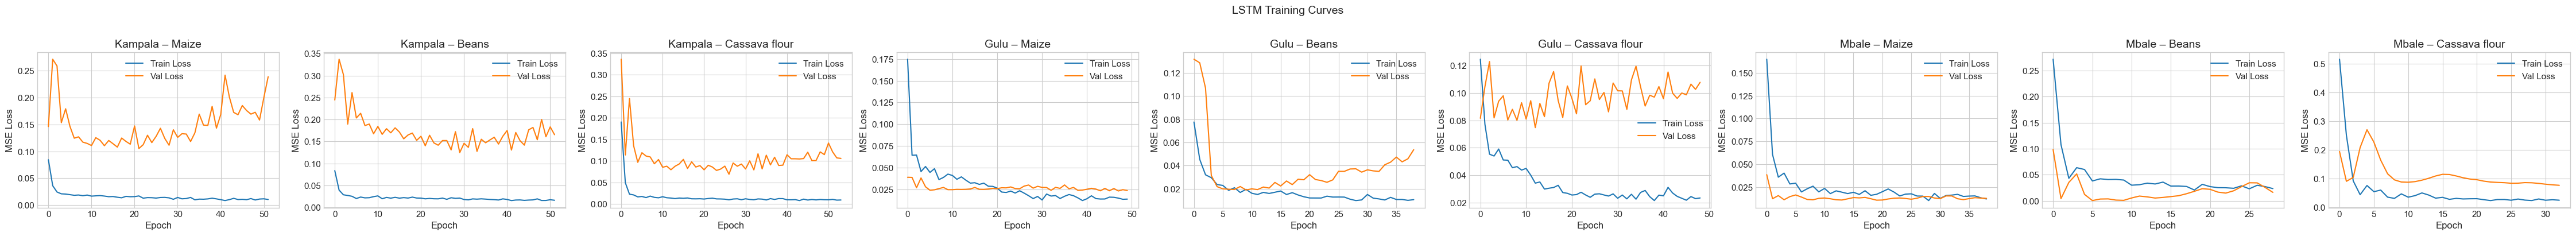
\includegraphics[width=\textwidth]{slides_img/plot_12.png}
\end{center}
\vspace{-0.2cm}
\footnotesize\textit{Training loss curves -- early stopping prevents overfitting on small dataset}
\end{column}
\begin{column}{0.48\textwidth}
\begin{center}
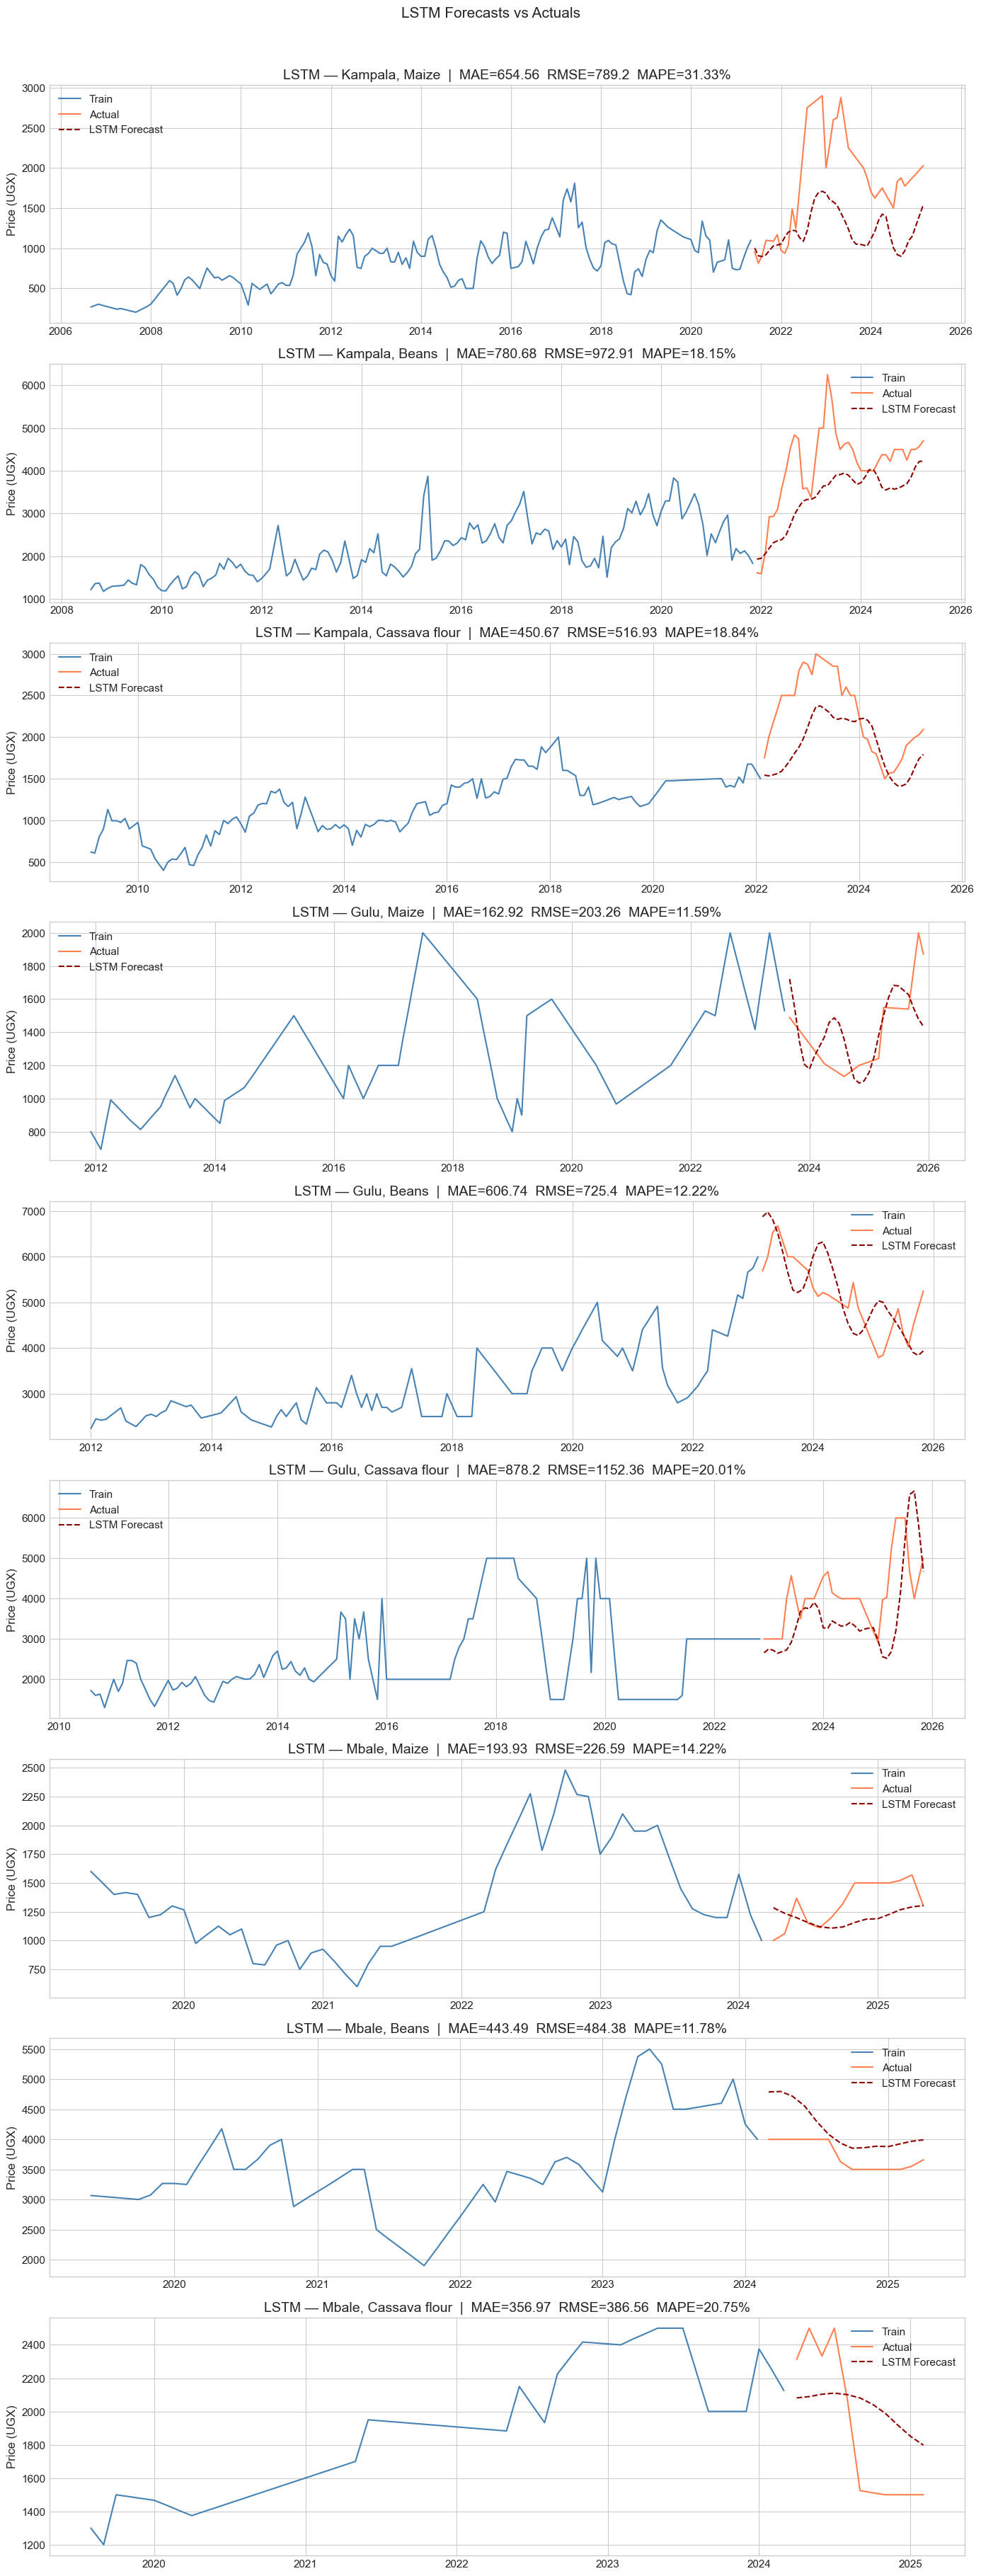
\includegraphics[width=\textwidth]{slides_img/plot_13.png}
\end{center}
\vspace{-0.2cm}
\footnotesize\textit{LSTM forecasts vs actuals -- average MAPE: \textbf{17.65\%} (best)}
\end{column}
\end{columns}
\end{frame}

% ============================================================
% SECTION 7: RESULTS (Presenter 4 - Barbra)
% ============================================================
\section{Results \& Model Comparison}

\begin{frame}{Evaluation Metrics}
\textit{\small Presenter: Apilli Barbra Ebal \hfill [22:00 -- 23:00]}
\begin{columns}
\begin{column}{0.33\textwidth}
\begin{block}{MAE}
$$\frac{1}{n}\sum|y_i - \hat{y}_i|$$
\centering Average error in UGX\\
\textit{Most interpretable}
\end{block}
\end{column}
\begin{column}{0.33\textwidth}
\begin{block}{RMSE}
$$\sqrt{\frac{1}{n}\sum(y_i - \hat{y}_i)^2}$$
\centering Penalises large errors\\
\textit{Sensitive to outliers}
\end{block}
\end{column}
\begin{column}{0.33\textwidth}
\begin{block}{MAPE}
$$\frac{100\%}{n}\sum\!\left|\frac{y_i - \hat{y}_i}{y_i}\right|$$
\centering Scale-independent\\
\textit{Cross-crop comparison}
\end{block}
\end{column}
\end{columns}

\vspace{0.8em}
\begin{block}{Evaluation Protocol}
\centering
Strict chronological \textbf{80/20 split} -- no shuffling $\rightarrow$ no data leakage $\rightarrow$ no future information in training
\end{block}
\end{frame}

\begin{frame}{Aggregate Results: LSTM Dominates}
\textit{\small Presenter: Apilli Barbra Ebal \hfill [23:00 -- 24:30]}
\begin{columns}
\begin{column}{0.45\textwidth}
\begin{table}
\centering
\begin{tabular}{lccc}
\toprule
\textbf{Model} & \textbf{MAE} & \textbf{RMSE} & \textbf{MAPE} \\
\midrule
\textcolor{arimaBlue}{ARIMA} & 757 & 882 & 25.1\% \\
\textcolor{prophetRed}{Prophet} & 841 & 970 & 29.7\% \\
\textcolor{lstmGreen}{\textbf{LSTM}} & \textcolor{lstmGreen}{\textbf{503}} & \textcolor{lstmGreen}{\textbf{606}} & \textcolor{lstmGreen}{\textbf{17.7\%}} \\
\bottomrule
\end{tabular}
\end{table}

\begin{block}{\small Why LSTM Wins}
\begin{enumerate}
    \small
    \item \textbf{Nonlinear} modelling capacity
    \item \textbf{Multivariate} (9 features vs 1)
    \item \textbf{Long-range memory} via gating
\end{enumerate}
\end{block}
\end{column}
\begin{column}{0.52\textwidth}
\begin{center}
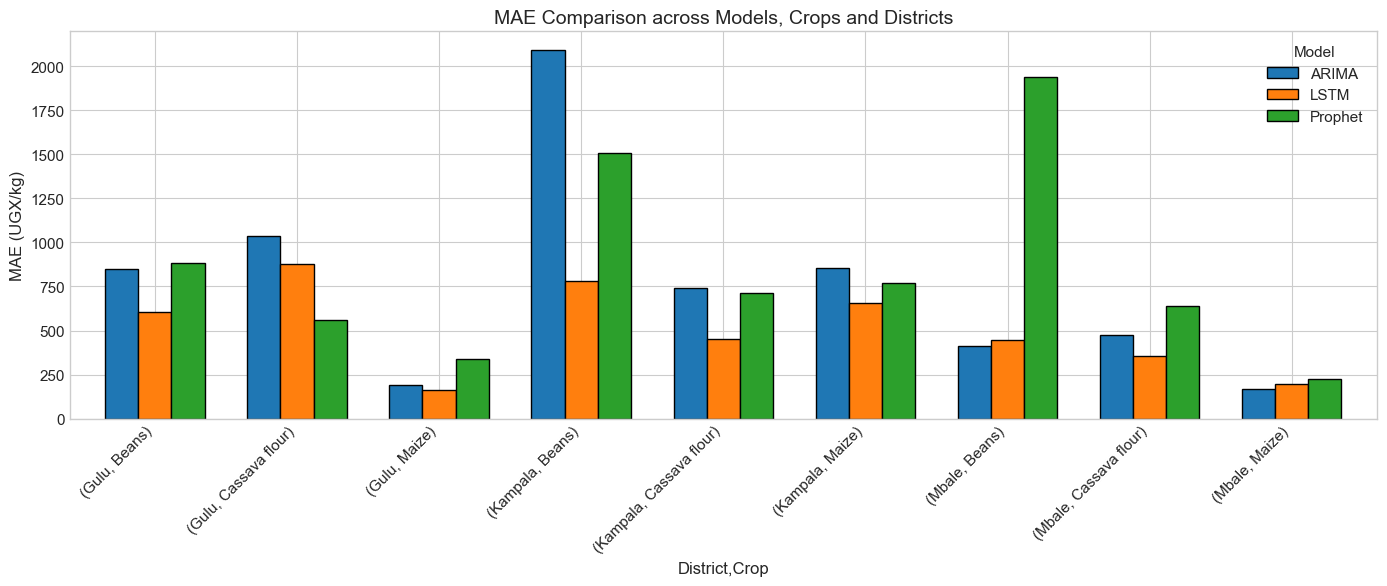
\includegraphics[width=\textwidth]{slides_img/plot_14.png}
\end{center}
\vspace{-0.3cm}
\footnotesize\textit{MAE comparison -- LSTM is \textbf{33\% lower} than ARIMA}
\end{column}
\end{columns}
\end{frame}

\begin{frame}{MAPE Comparison \& All-Models Overlay}
\textit{\small Presenter: Apilli Barbra Ebal \hfill [24:30 -- 25:30]}
\begin{columns}
\begin{column}{0.48\textwidth}
\begin{center}
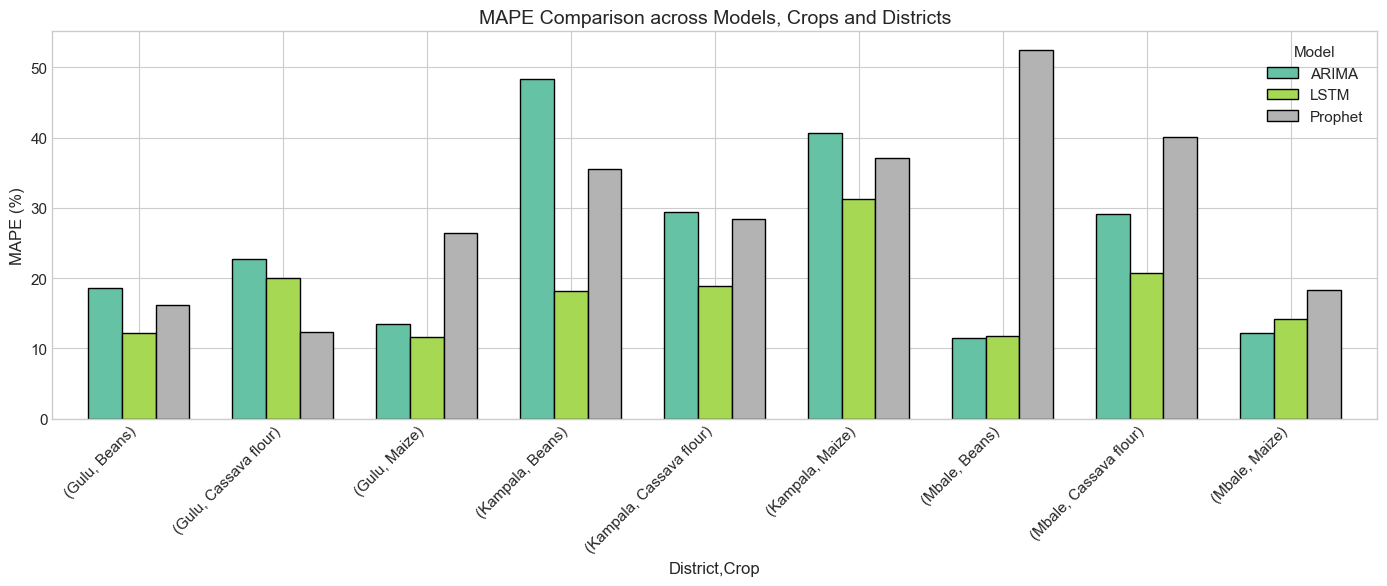
\includegraphics[width=\textwidth]{slides_img/plot_15.png}
\end{center}
\vspace{-0.2cm}
\footnotesize\textit{MAPE comparison -- LSTM best in 7/9 pairs}
\end{column}
\begin{column}{0.48\textwidth}
\begin{center}
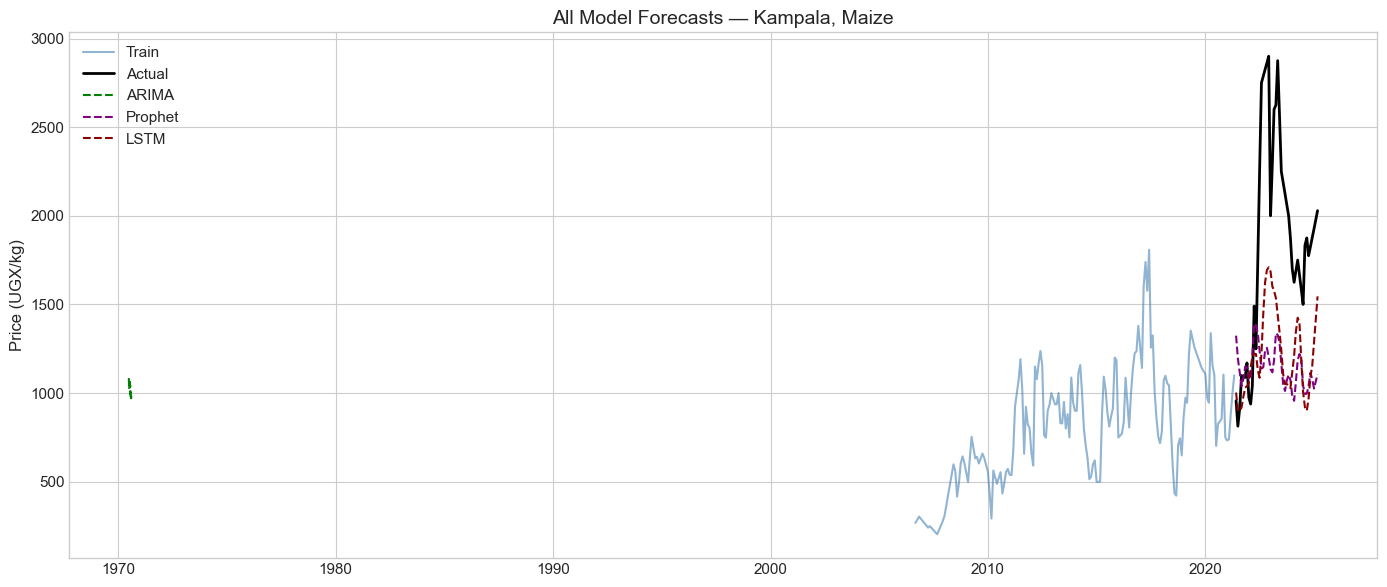
\includegraphics[width=\textwidth]{slides_img/plot_16.png}
\end{center}
\vspace{-0.2cm}
\footnotesize\textit{All three models overlaid -- LSTM (green) tracks actuals most closely}
\end{column}
\end{columns}
\end{frame}

\begin{frame}{District-Level Performance Breakdown}
\textit{\small Presenter: Apilli Barbra Ebal}
\begin{table}
\centering
\footnotesize
\begin{tabular}{llccc}
\toprule
\textbf{District} & \textbf{Crop} & \textbf{ARIMA MAPE} & \textbf{Prophet MAPE} & \textbf{LSTM MAPE} \\
\midrule
Kampala & Maize & 40.66\% & 37.13\% & \textcolor{lstmGreen}{\textbf{31.33\%}} \\
Kampala & Beans & 48.35\% & 35.59\% & \textcolor{lstmGreen}{\textbf{18.15\%}} \\
Kampala & Cassava flour & 29.40\% & 28.40\% & \textcolor{lstmGreen}{\textbf{18.84\%}} \\
\midrule
Gulu & Maize & 13.49\% & 26.39\% & \textcolor{lstmGreen}{\textbf{11.59\%}} \\
Gulu & Beans & 18.60\% & 16.18\% & \textcolor{lstmGreen}{\textbf{12.22\%}} \\
Gulu & Cassava flour & 22.67\% & \textcolor{prophetRed}{\textbf{12.34\%}} & 20.01\% \\
\midrule
Mbale & Maize & \textcolor{arimaBlue}{\textbf{12.25\%}} & 18.37\% & 14.22\% \\
Mbale & Beans & \textcolor{arimaBlue}{\textbf{11.52\%}} & 52.50\% & 11.78\% \\
Mbale & Cassava flour & 29.08\% & 40.07\% & \textcolor{lstmGreen}{\textbf{20.75\%}} \\
\bottomrule
\end{tabular}
\end{table}
\vspace{0.3em}
\centering \footnotesize
\textcolor{lstmGreen}{\textbf{LSTM wins 7/9}} $\bullet$ \textcolor{arimaBlue}{\textbf{ARIMA wins 2/9}} (Mbale -- simpler, stable market) $\bullet$ \textcolor{prophetRed}{\textbf{Prophet wins 1/9}} (strong annual seasonality)
\end{frame}

% ============================================================
% SECTION 8: DASHBOARD (Presenter 4 continued)
% ============================================================
\section{Streamlit Dashboard}

\begin{frame}[fragile]{Interactive Web Dashboard: Live Demo}
\textit{\small Presenter: Apilli Barbra Ebal \hfill [25:00 -- 27:30]}
\begin{columns}
\begin{column}{0.55\textwidth}
\textbf{Dashboard Features:}
\begin{enumerate}
    \item \textbf{User Controls:} Select crop, district, horizon
    \item \textbf{Real-time LSTM Training:} Model trains live
    \item \textbf{Interactive Plotly Chart:}
    \begin{itemize}
        \item Historical train data
        \item Test actuals vs LSTM predictions
        \item Future forecast trajectory
    \end{itemize}
    \item \textbf{Performance Metrics:} MAE, RMSE, MAPE
    \item \textbf{Model Comparison Panel}: ARIMA vs Prophet vs LSTM
\end{enumerate}

\vspace{0.5em}
\begin{lstlisting}
# Launch command
streamlit run app.py
\end{lstlisting}
\end{column}
\begin{column}{0.42\textwidth}
\begin{lstlisting}
# Dashboard core: app.py
import streamlit as st
import tensorflow as tf

st.title("Deep Market Forecaster")

# User selects parameters
district = st.selectbox(
    "District:",
    ['Kampala','Gulu','Mbale'])
crop = st.selectbox(
    "Crop:",
    ['Maize','Beans',
     'Cassava flour'])
horizon = st.radio(
    "Forecast Horizon:",
    ["4 Weeks", "8 Weeks"])

# Generate button triggers
# LSTM training + forecasting
if st.button("Generate Forecast"):
    model = train_lstm(data)
    forecast = predict(model)
    st.plotly_chart(fig)
\end{lstlisting}
\end{column}
\end{columns}
\end{frame}

% ============================================================
% SECTION 9: CHALLENGES & CONCLUSIONS (Presenter 4)
% ============================================================
\section{Challenges \& Conclusions}

\begin{frame}{Challenges Faced \& Overcome}
\textit{\small Presenter: Apilli Barbra Ebal \hfill [27:30 -- 29:00]}
\begin{columns}
\begin{column}{0.48\textwidth}
\begin{block}{1. Data Sparsity}
\textbf{Problem:} Neural networks need 10,000+ rows; we had $\sim$200\\
\textbf{Solution:}
\begin{itemize}
    \item \textbf{Dropout} (20\%) -- implicit ensemble
    \item \textbf{Early stopping} (patience=10)
    \item Compact architecture (64$\rightarrow$32)
\end{itemize}
\end{block}

\begin{block}{2. Geographic Mismatch}
\textbf{Problem:} WFP $\neq$ CHIRPS $\neq$ World Bank\\
\textbf{Solution:} Manual mapping dicts + MS resampling
\end{block}
\end{column}
\begin{column}{0.48\textwidth}
\begin{block}{3. Multi-step Forecasting}
\textbf{Problem:} Error compounds recursively\\
\textbf{Solution:} Recursive strategy with lag updates
\end{block}

\begin{alertblock}{Known Limitations}
\begin{itemize}
    \item Single train/test split (vs time-series CV)
    \item No confidence intervals
    \item ARIMA used univariate only
    \item Cannot predict black swan events
\end{itemize}
\end{alertblock}
\end{column}
\end{columns}
\end{frame}

\begin{frame}{Conclusions \& Future Work}
\textit{\small Presenter: Apilli Barbra Ebal \hfill [29:00 -- 30:00]}
\begin{block}{What We Achieved}
\begin{enumerate}
    \item Built \textbf{end-to-end ML pipeline}: data $\rightarrow$ features $\rightarrow$ models $\rightarrow$ evaluation $\rightarrow$ deployment
    \item Merged \textbf{3 heterogeneous datasets} (WFP + CHIRPS + World Bank)
    \item Trained and compared \textbf{3 fundamentally different models}
    \item LSTM achieved \textbf{17.65\% average MAPE} -- competitive with published benchmarks
    \item Deployed to \textbf{interactive Streamlit dashboard} with model comparison panel
\end{enumerate}
\end{block}

\begin{block}{Future Work}
\begin{columns}
\begin{column}{0.48\textwidth}
\begin{itemize}
    \item Transformer architectures
    \item Model ensembling (learned weights)
    \item Additional covariates (conflict, mobility)
\end{itemize}
\end{column}
\begin{column}{0.48\textwidth}
\begin{itemize}
    \item Probabilistic forecasts (intervals)
    \item Cloud deployment (AWS/GCP)
    \item SMS/USSD for farmer access
\end{itemize}
\end{column}
\end{columns}
\end{block}
\end{frame}

% ============================================================
% THANK YOU
% ============================================================
\begin{frame}{}
\centering
\vspace{1.5cm}
{\Huge\textbf{Thank You}}\\[0.8em]
{\Large Questions \& Discussion}\\[1.5em]
\begin{tabular}{ll}
\textbf{Repository:} & \url{https://github.com/Jamugisa-Peter-Paul/Price-forcasting} \\
\textbf{Dashboard:} & \texttt{streamlit run app.py} \\
\end{tabular}\\[1.5em]
\rule{8cm}{0.5pt}\\[0.5em]
\small Jamugisa Peter Paul $\bullet$ ILEGO Cynthia Cecilia $\bullet$ AYEBARE Moses $\bullet$ Apilli Barbra Ebal
\end{frame}

\end{document}
